\chapter[Modeling the core circadian feedback loop to determine the effect of KL001]{Modeling the core circadian feedback loop to determine the effect of KL001\footnote{ Portions of this chapter are published in T. Hirota, J. W. Lee, P. C. St. John, M. Sawa, K. Iwaisako, T. Noguchi, P. Y. Pongsawakul, T. Sonntag, D. K. Welsh, D. A. Brenner, F. J. Doyle, P. G. Schultz, and S. A. Kay, ``Identification of Small Molecule Activators of Cryptochrome.,'' {\itshape Science}, vol. 337, pp. 1094–1097, July 2012.}}\label{chap:model}

\section{Background}

\subsection{Small molecule modulators}
Circadian rhythms help to regulate metabolic homeostasis, and therefore compromised circadian oscillations often result in negative health consequences.
Since circadian rhythms may be damped by lifestyle factors, many researchers have begun searching for pharmacological agents which might alter circadian rhythmicity.
Several proof-of-concept molecules have been found which cause dose-dependent period change in cultured fibroblasts \cite{Chen2013}.
While chemical biology approaches are able to localize the effects of these molecules to specific targets in the circadian network, it is often difficult to reconcile individual rate changes with the observed systems-level changes in period or amplitude.
Mathematical models are therefore essential to understanding the effects of such drugs, as they are able to verify that hypothesized mechanisms of action are mathematically consistent.
Furthermore, mathematical models provide a systematic framework by which to examine consequences of various mechanistic assumptions - many of which can be subsequently verified by experimental inquiry.
The search for small molecule modulators of circadian rhythms therefore yields the added benefit of strengthening our knowledge of the core clock feedback circuit, as inconsistencies between assumed kinetics and experimental results often lead to a more refined knowledge of the network's dynamics.

In this chapter, we describe a collaborative project in which experimental results inspired the creation of a new model of the core mammalian feedback network.
A new small molecule modulator of cryptochrome, KL001, was identified through forward chemical genetic screening \cite{Hirota2012}.
The compound was found to simultaneously increase the half-life of CRY and cause period lengthening.
In order to explain these new experimental results while maintaining consistency with published evidence, we constructed a simple mathematical model of the PER/CRY negative feedback loop.

The functional roles of the cryptochrome isoforms ({\it Cry1} and {\it Cry2}) in circadian rhythms have long eluded biologists, as although they share a similar structure, perturbations to these genes typically result in opposite trends \cite{McCarthy2009}.
Existing genetic evidence and siRNA knockdown studies agree that while suppressing {\it Cry1} leads to shorter periods, suppressing {\it Cry2} leads to longer periods \cite{VanderHorst1999, Zhang2009}.
However, some evidence shows the similarity between the two {\it Crys}.
The knockouts\footnote{Wild type mammals, denoted with the ``$+/+$'' superscript, receive two copies of every gene from each parent. Homozygous knockouts, denoted ``$-/-$'', have no functional copies of the gene. Heterozygous knockouts, denoted ``$+/-$'', receive only one functional copy and therefore express the gene at lower levels.} $\text{\it Cry1}^{+/-}$ $\text{\it Cry2}^{-/-}$ and $\text{\it Cry1}^{-/-}$ $\text{\it Cry2}^{+/-}$ both show shorter wheel-running activity their respective WT/double knockouts $\text{\it Cry1}^{+/+}$ $\text{\it Cry2}^{-/-}$ and $\text{\it Cry1}^{-/-}$ $\text{\it Cry2}^{+/+}$ \cite{VanderHorst1999}.
Using new data from the application of KL001 together with existing experimental results, we developed a hypothesized mechanism to reconcile these seemingly contradictory results:

\subsubsection{Network structure}
In the core feedback loop, {\itshape Per} and {\itshape Cry} transcription is activated by the CLOCK-BMAL1 complex.
The protein products of these genes are transported to the nucleus after a time delay and bind to CLOCK-BMAL1, repressing their own transcription.
Evidence indicates that an interaction of PER and CRY proteins is required for the timely nuclear entry of both proteins \cite{Miyazaki2001,Ko2006,Kume1999}.
We therefore assume that PER and CRY bind and enter the nucleus in a 1:1 stoichiometric ratio, similar to more complicated models of mammalian circadian rhythms \cite{Leloup2003,Mirsky2009,Forger2003}.

\subsubsection{Protein stoichiometry}
Quantitative protein assays have revealed that the PER proteins are present at levels nearly ten times less than the CRYs, and are completely consumed at their trough.
The CRYs, on the other hand, only fall to about one quarter of their peak value  \cite{Lee2001}.
These results indicate that PER is the rate-limiting component for nuclear entry.
This configuration explains why, since {\itshape Cry} is in excess, a knockout of either {\it Cry} alone does not lead to loss of function at the tissue level.
Additionally CRY1, the more dominant repressor, is consistently found at higher levels than CRY2.
However, since the ratio of nuclear to total protein is nearly equivalent for CRY1 and CRY2, PER must import each with equal affinity \cite{Lee2001,Lee2011b}.

\subsubsection{Importance of degradation}
Studies of the simplest cellular oscillators have illustrated the importance of the degradation of repressor complexes in determining the period of oscillation \cite{Cookson2009}.
In the mammalian circadian clock, FBXL3 has been indicated as a key protein in clearing the nucleus of CRY, and siRNA knockdowns of {\it Fbxl3} result in period lengthening \cite{Zhang2009}.
While FBXL3 localizes primarily in the nucleus, CRY2 possesses a distinct phosphorylation domain that flags it for cytosolic proteolysis \cite{Kurabayashi2010}.
Knocking down this domain shortens the period, indicating that degradation rates play a major role in determining the oscillatory period and that stabilization in the cytosol and nucleus are likely not equivalent.

\subsubsection{Key time delays}
Similar to {\it Drosophila}, mammalian circadian oscillations are generated by three main time delays in the negative feedback loop: mRNA transcription, nuclear localization of protein, and degradation of the nuclear complexes \cite{Vielhaber2000a}.
In order to capture these dynamics without introducing unnecessary stiffness, we explicitly consider only the concentrations of nuclear mRNA, cytosolic unbound protein, and nuclear protein complexes.

\section{Results}

\subsection{A new model for period regulation}
Since the circadian clock is largely insensitive to the total amount {\it Cry}, it follows that the core negative loop is comprised of two redundant coupled inhibitory mechanisms. 
The natural periods of these two loops (running in isolation of the other) can be inferred from their corresponding knockout phenotype, i.e., the CRY1 feedback loop has a long period, while the CRY2 loop has a short period. 
In the wild-type phenotype, the two isoforms of CRY must compete for the available PER, and thus the nuclear CRY1/CRY2 levels are constrained with a ratio proportional to their relative expression. 
This suggests that the period of the clock is governed by the nuclear CRY1/CRY2 ratio, where higher amounts of {\it Cry1} shift the clock closer to the $\text{\it Cry2}^{-/-}$ phenotype, and higher amounts of {\it Cry2} shift the clock closer to the $\text{\it Cry1}^{-/-}$ phenotype, described in \fref{fig:twoloops}.

\begin{figure}[bt]
  \centering
  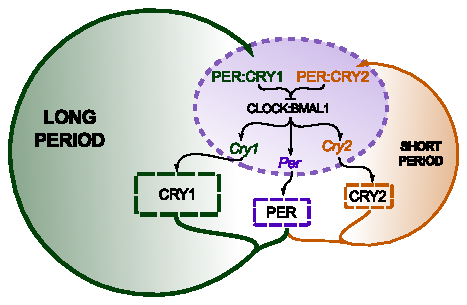
\includegraphics[width=0.8\textwidth]{chap2/figures/twoloops_noopacity.pdf}
  \titlecaption{Connectivity of \fref{mod:hirota}}{
    Schematic for the core negative feedback loop, consisting of the two redundant {\it Cry} mechanisms. 
  The wild-type period, consisting of both loops, is a balance between the short and long oscillations.} \label{fig:twoloops}
\end{figure}

\subsubsection{The CRY1/CRY2 ratio}
{\it In silico} modeling was used to test the feasibility of the above hypothesis, and to investigate possible mechanisms by which the CRY1/CRY2 ratio might control the period of oscillations. 
The model uses eight state variables for the three mRNA species ({\it Per}, {\it Cry1}, and {\it Cry2}), three cytosolic proteins, and two nuclear proteins. 
The differential equations for each state were formulated using standard Hill-type repression, Michaelis-Menten, and mass action kinetics. 
The 21 unknown kinetic parameters were found by fitting the stoichiometric data from \cite{Lee2001} using a genetic algorithm approach, requiring correct periods for the $\text{\it Cry1}^{-/-}$  and $\text{\it Cry2}^{-/-}$  knockouts.

We investigated two possible mechanisms to explain the long/short period phenotype of the CRY1/CRY2 loops. 
First, following experimental evidence, we allowed CRY1 and CRY2 to have different inhibitory efficiency \cite{GriffinJr.1999}. 
However, optimizations with this structure were unable to find a parameter set with appropriate period sensitivities, described in \fref{sec:parameter}. 
Instead, we investigated whether the difference in potency between {\it Crys} could be explained through difference in degradation rates. 
To this end, we allowed the degradation rates of nuclear CRY1 and CRY2 to differ, while holding their inhibition constants equal. 
Using this configuration, the structure was able to fit the experimental sensitivities. 
In the optimized parameter set, the degradation rate of nuclear CRY2 is higher than that of CRY1, such that for a constant total nuclear CRY, higher fractions of CRY2 cause the repressive complexes to be cleared faster. 
Since PER is the limiting reagent in nuclear entry, the amount of total CRY that enters the nucleus is largely insensitive to perturbations in cytosolic CRY expression. 
In effect, the two isoforms of CRY must compete for the available PER, and thus the nuclear CRY1/CRY2 levels are constrained with a ratio proportional to their relative expression. 
The period of the clock is thus governed by the nuclear CRY1/CRY2 ratio, where higher amounts of {\it Cry1} shift the clock closer to the $\text{\it Cry2}^{-/-}$ phenotype, and higher amounts of {\it Cry2} shift the clock closer to the $\text{\it Cry1}^{-/-}$ phenotype. 
\Fref{fig:nucleartimecourse} shows the time varying total complex concentration under various perturbations, with the relative contributions from CRY1 and CRY2 highlighted.

\begin{figure}[bt]
  \centering
  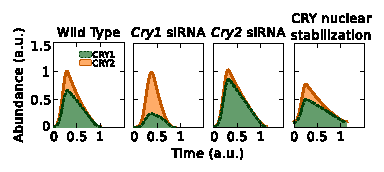
\includegraphics[width=0.8\textwidth]{chap2/figures/nucleartimecourse.pdf}
  \titlecaption{Repressor degradation profiles}{
    Time course plots of the simulated total nuclear repressor concentration for the degradation model under various clock conditions. 
    The relative contribution of CRY1 and CRY2 are shaded green and orange, respectively. 
  Longer periods occur when a higher percentage of the nuclear complex is CRY1, taking longer to degrade.}
  \label{fig:nucleartimecourse}
\end{figure}

\subsubsection{Model equations}
The model is formulated as set of 8 ordinary differential equations shown in \fref{mod:hirota} (for the degradation-based model) and \fref{mod:actfns} (for the activation-based model). 
Additional assumptions made while formulating the model equations are listed below:

\begin{itemize}

  \item For simplicity and  ease of parameter estimation, the model only considers the three genes {\it Per}, {\it Cry1}, and {\it Cry2}, not explicitly considering the three known isoforms of {\it Per}. 

  \item EBOX activators {\it Clock} and {\it Bmal1} are considered constitutively expressed and are represented by the $v_{\text{txn}}$ parameters. 

  \item Repression of CLOCK-BMAL1 activity is attained through Hill-type inhibition. The Hill coefficient is fixed at 3, which was found to provide sufficient nonlinearity for oscillations. See below for the derivation of the repressor input function used in \fref{mod:hirota} and \fref{mod:actfns}.

  \item The degradation of the mRNA species and cytoplasmic proteins is assumed to follow standard Michaelis-Menten kinetics.

  \item The degradation kinetics of the nuclear proteins are assumed to follow Michaelis-Menten kinetics. Because both $\bm{C1N}$ and $\bm{C2N}$ are thought to be degraded by the same pathway in the nucleus, kinetic equations using the {\it pseudo} steady-state hypothesis were derived for two substrates sharing the same enzyme. As a result, each CRY isoform acts as an inhibitor to the other's degradation. This mechanism is summarized in \fref{fig:shareddeg}.
\end{itemize}

\begin{figure}[tbp]
  \centering
  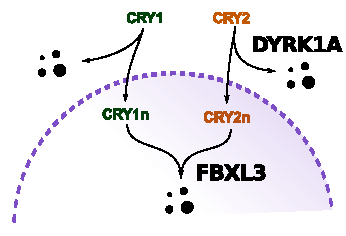
\includegraphics{chap2/figures/cryseperatedegradation.pdf}
  \titlecaption{Degradation of both CRY isoforms is regulated by the same enzyme}{In developing the model equations for \fref{mod:hirota}, a key assumption was that both isoforms of Cryptochrome were degraded by the same enzyme. Without such a scheme, the shortest periods were obtained by maximizing degradation through equal nuclear entry of both isoforms.}
  \label{fig:shareddeg}
\end{figure}

\begin{model}[p]
  \centering
  \titlecaption{A degradation-based model of the core feedback loop}{Lower case letters (p: {\it Per}, c1: {\it Cry1}, c2: {\it Cry2}) are mRNA state variables. Uppercase letters (P: PER, C1: CRY1, C2: CRY2) are the free (cytosolic) proteins. C1N: CRY1 and C2N: CRY2 are the nuclear proteins.}

  \begin{align}
    \label{eq:p}
    \frac{d\mathrm{\bf p}}{dt}    & = \frac{v_{\text{txn,{\bf p}}}}{k_{\text{txn,{\bf p}}} + \left(\text{\bf C1N} + \text{\bf C2N} \right)^3} - \frac{v_{\text{deg,{\bf p}}} \;\text{\bf p} }{k_{\text{deg,{\bf p}}} +\text{\bf p} } \\
        %
    \label{eq:c1}
    \frac{d\text{\bf c1}}{dt}   & = \frac{v_{\text{txn,{\bf c1}}}}{k_{\text{txn,{\bf c}}} + \left(\text{\bf C1N} + \text{\bf C2N} \right)^3} - \frac{v_{\text{deg,{\bf c1}}} \;\text{\bf c1} }{k_{\text{deg,{\bf c}}} +\text{\bf c1} } \\
        %
    \label{eq:c2}
    \frac{d\text{\bf c2}}{dt}   & = \frac{v_{\text{txn,{\bf c2}}}}{k_{\text{txn,{\bf c}}} + \left(\text{\bf C1N} + \text{\bf C2N} \right)^3} - \frac{v_{\text{deg,{\bf c2}}} \;\text{\bf c2} }{k_{\text{deg,{\bf c}}} +\text{\bf c2} } \\
        %
    \begin{split}
      \frac{d\text{\bf P}}{dt}  & = k_\text{tln,{\bf p}} \;\text{\bf p}  - \frac{v_{\text{deg,{\bf P}}} \;\text{\bf P} }{k_{\text{deg,{\bf P}}} +\text{\bf P} } - v_{\text{a,{\bf CP}}} \;\text{\bf P}  \;\text{\bf C1}  + v_{\text{d,{\bf CP}}} \;\text{\bf C1N} \\
      & \quad - v_{\text{a,{\bf CP}}} \;\text{\bf P}  \;\text{\bf C2}  + v_{\text{d,{\bf CP}}} \; \text{\bf C2N}
    \end{split} \\
        %
    \frac{d\text{\bf C1}}{dt}   & =\text{\bf c1}  - \frac{v_{\text{deg,{\bf C1}}} \;\text{\bf C1} }{k_{\text{deg,{\bf C}}} +\text{\bf C1} } - v_{\text{a,{\bf CP}}} \;\text{\bf P}  \;\text{\bf C1}  + v_{\text{d,{\bf CP}}} \;\text{\bf C1N} \\
        %
    \frac{d\text{\bf C2}}{dt}   & =\text{\bf c2} - \frac{ v_{\text{deg,{\bf C2}}} \;\text{\bf C2} }{k_{\text{deg,{\bf C}}} +\text{\bf C2} } - v_{\text{a,{\bf CP}}} \;\text{\bf P}  \;\text{\bf C2}  + v_{\text{d,{\bf CP}}} \; \text{\bf C2N} \\
        %
    \frac{d\text{\bf C1N}}{dt}  & = - \frac{ v_{\text{deg,{\bf CP}}} \;\text{\bf C1N} }{k_{\text{deg,{\bf CP}}} +\text{\bf C1N}  + \text{\bf C2N} } + v_{\text{a,{\bf CP}}} \;\text{\bf P}  \;\text{\bf C1} - v_{\text{d,{\bf CP}}} \;\text{\bf C1N} \\
        %
    \label{eq:C2N}
    \frac{d\text{\bf C2N }}{dt} & = - \frac{ \left(v_{\text{deg,{\bf CP}}} \; m_{\text{\bf C2N}}\right) \; \text{\bf C2N} }{k_{\text{deg,{\bf CP}}} + \text{\bf C2N}  +\text{\bf C1N} } + v_{\text{a,{\bf CP}}} \;\text{\bf P}  \;\text{\bf C2} - v_{\text{d,{\bf CP}}} \; \text{\bf C2N}
  \end{align}
  \label{mod:hirota}
\end{model}


\begin{model}[p]
  \centering
  \titlecaption{Changed equations for the activation-based model}{The remainder of the model equations (not duplicated below) are found in  \fref{mod:hirota}}

  \begin{align*}
    \frac{d\text{\bf p}}{dt} &= \frac{v_{\text{txn,{\bf p}}}}{k_{\text{txn,{\bf p}}} + \left(m_{\text{\bf C2N}} \; \text{\bf C1N}  + \text{\bf C2N} \right)^3} - \frac{v_{\text{deg,{\bf p}}} \;\text{\bf p} }{k_{\text{deg,{\bf p}}} +\text{\bf p} } \tag{$\ref{eq:p}^{\star}$}\\
        %
    \frac{d\text{\bf c1}}{dt} &= \frac{v_{\text{txn,{\bf c1}}}}{k_{\text{txn,{\bf c}}} + \left(m_{\text{\bf C2N}} \; \text{\bf C1N}  + \text{\bf C2N} \right)^3} - \frac{v_{\text{deg,{\bf c1}}} \;\text{\bf c1} }{k_{\text{deg,{\bf c}}} +\text{\bf c1} } \tag{$\ref{eq:c1}^{\star}$}\\
        %
    \frac{d\text{\bf c2}}{dt} &= \frac{v_{\text{txn,{\bf c2}}}}{k_{\text{txn,{\bf c}}} + \left(m_{\text{\bf C2N}} \; \text{\bf C1N}  + \text{\bf C2N} \right)^3} - \frac{v_{\text{deg,{\bf c2}}} \;\text{\bf c2} }{k_{\text{deg,{\bf c}}} +\text{\bf c2} } \tag{$\ref{eq:c2}^{\star}$}\\
        %
    \frac{d\text{\bf C2N }}{dt} &= - \frac{ v_{\text{deg,{\bf CP}}} \; \text{\bf C2N} }{k_{\text{deg,{\bf CP}}} + \text{\bf C2N}  +\text{\bf C1N} } + v_{\text{a,{\bf CP}}} \;\text{\bf P}  \;\text{\bf C2} - v_{\text{d,{\bf CP}}} \; \text{\bf C2N}
    \tag{$\ref{eq:C2N}^{\star}$}
  \end{align*}
  \label{mod:actfns}
\end{model}


\begin{table}[p]
  \titlecaption{Parameter values for \fref{mod:hirota}}{Parameters for model described in \fref{mod:hirota}.}
  \label{tab:parset}
  \vspace{2mm}
  \centering
  \begin{tabular}{cllrr} \toprule
    & Parameter                 & Description                       & Degradation & Activation \\ \midrule
    1  & $v_{\text{txn,{\bf p}}}$  & {\it Per} Transcription rate      & 0.195       & 0.276 \\
    2  & $v_{\text{txn,{\bf c1}}}$ & {\it Cry1} Transcription rate     & 0.131       & 0.062 \\
    3  & $v_{\text{txn,{\bf c2}}}$ & {\it Cry1} Transcription rate     & 0.114       & 0.053 \\
    4  & $k_{\text{txn,{\bf p}}}$  & {\it Per} Repression constant     & 0.425       & 0.425 \\
    5  & $k_{\text{txn,{\bf c}}}$  & {\it Cry1/2} Repression constant  & 0.259       & 0.262 \\
    6  & $v_{\text{deg,{\bf p}}}$  & {\it Per} Max degradation rate    & 0.326       & 0.472 \\
    7  & $v_{\text{deg,{\bf c1}}}$ & {\it Cry1} Max degradation rate   & 0.676       & 0.322 \\
    8  & $v_{\text{deg,{\bf c2}}}$ & {\it Cry2} Max degradation rate   & 0.608       & 0.290 \\
    9  & $k_{\text{deg,{\bf p}}}$  & {\it Per} Degradation constant    & 0.011       & 0.024 \\
    10 & $k_{\text{deg,{\bf c}}}$  & {\it Cry1/2} Degradation constant & 1.149       & 0.809 \\
    11 & $v_{\text{deg,{\bf P}}}$  & Max PERc degradation rate         & 2.970       & 2.970 \\
    12 & $k_{\text{deg,{\bf P}}}$  & PERc degradation constant         & 0.034       & 0.034 \\
    13 & $v_{\text{deg,{\bf C1}}}$ & Max CRY1c degradation rate        & 1.523       & 1.048 \\
    14 & $v_{\text{deg,{\bf C2}}}$ & Max CRY2c degradation rate        & 1.686       & 1.134 \\
    15 & $k_{\text{deg,{\bf C}}}$  & CRYc degradation constant         & 2.017       & 2.028 \\
    16 & $v_{\text{deg,{\bf CP}}}$ & CRYn degradation rate             & 0.101       & 0.070 \\
    17 & $m_{\text{\bf C2N}}$      & CRY2n degradation multiplier      & 3.318       & 3.334 \\
    18 & $k_{\text{deg,{\bf CP}}}$ & CRYn degradation constant         & 0.053       & 0.053 \\
    19 & $v_{\text{a,{\bf CP}}}$   & CRYn association rate             & 0.041       & 0.028 \\
    20 & $v_{\text{d,{\bf CP}}}$   & CRYn dissociation rate            & 0.002       & 0.001 \\
    21 & $k_{\text{tln,{\bf p}}}$  & PER translation rate              & 3.000       & 1.000 \\ \bottomrule
    \hline
  \end{tabular}
\end{table}


\subsubsection{Derivation of a shared enzyme degradation rate}

To find the rate equations associated with a shared-enzyme degradation mechanism, we derive them from the equilibrium relationships:
\begin{equation*}
  \text{[E]} + \text{[S1]} \xrightleftharpoons[k_{-1}]{k_1} \text{[ES1]} \xrightarrow{k_{d,1}} \text{[E]}
\end{equation*}
\begin{equation*}
  \text{[E]} + \text{[S2]} \xrightleftharpoons[k_{-2}]{k_2}  \text{[ES2]} \xrightarrow{k_{d,2}} \text{[E]}
\end{equation*}
\begin{equation} \label{eq:totE}
  [\text{E}_t] = \text{[E]} + \text{[ES1]} + \text{[ES2]}
\end{equation}
The end goal is the degradation rates of the two enzyme complexes:
\begin{align}
  \begin{split}\label{eq:r1}
    r_{d,1} &= k_{d,1} \ \text{[ES1]}\\
    r_{d,2} &= k_{d,2} \ \text{[ES2]}
  \end{split}
\end{align}
As was done in \fref{sec:mmenten}, we invoke the standard pseudo steady-state assumption and set $\nicefrac{d[\text{ES}]}{dt}=0$, and obtain the following production = consumption equalities for [ES1]:
\begin{equation} \label{eq:pss}
  k_1\text{[E]}\text{[S]} = k_{-1}\text{[ES1]} + k_{d,1}\text{[ES1]}
\end{equation}
Solving \fref{eq:pss} for ES1 and substituting in \fref{eq:totE}, we obtain
\begin{equation*}
  \left(\frac{k_{-1}+k_{d,1}}{k_1}\right)\text{[ES1]} = \left([\text{E}_t] - \text{[ES1]} - \text{[ES2]}\right)\text{[S1]}
\end{equation*}
After defining a useful combined rate constant,
\begin{equation*}
  K_1 \equiv \frac{k_{-1}+k_{d,1}}{k_1}
\end{equation*}
we can further simplify
\begin{align}
  K_1 \text{[ES1]} + \text{[S1]}\text{[ES1]} &= ([\text{E}_t] - [\text{ES2}])[\text{S1}] \notag\\
    %
  [\text{ES1}] &= \frac{([\text{E}_t] - [\text{ES2}])[\text{S1}]}{K_1 + [\text{S1}]} \label{eq:eqabove}
\end{align}
If we perform the same operations for [ES2] and plug them into \fref{eq:eqabove}.
\begin{align}
  [\text{ES1}] &= \frac{\left(\text{E}_t] - \frac{([\text{E}_t] - [\text{ES1}])[\text{S2}]}{K_2 + [\text{S2}]}\right)\text{S1}]}{K_1 + [\text{S1}]} \notag\\
  [\text{ES1}] &= \frac{\text{[E]}_t \text{[S1]}}{K_1 + \text{[S1]}} - \frac{\text{[E]}_t \text{[S1]} \text{[S2]}}{(K_1 + \text{[S1]}) (K_2 + \text{[S2]})} + \frac{\text{[ES1]} \text{[S1]} \text{[S2]}}{(K_1 + \text{[S1]}) (K_2 + \text{[S2]})} \notag\\
  \label{eq:twofracs}
  [\text{ES1}] &= \left(\frac{\text{[E]}_t \text{[S1]}}{K_1 + \text{[S1]}}\right) \left(\frac{1 - \frac{\text{[S2]}}{K_2 + \text{[S2]}}}{1 - \frac{\text{[S1]} \text{[S2]}}{(K_1 + \text{[S1]}) (K_2 + \text{[S2]})}}\right)
\end{align}
If we pull the second fraction from \fref{eq:twofracs} into the denominator of the first, we can simplify further.
\begin{align*}
  [\text{ES1}] &= \frac{\text{[E]}_t \text{[S1]}}{\left(\frac{K_1 + \text{[S1]} - \frac{\text{[S1]} \text{[S2]}}{K_2 + \text{[S2]}}}{1 - \frac{\text{[S2]}}{K_2 + \text{[S2]}}}\right)} \\
  [\text{ES1}] &= \frac{\text{[E]}_t \text{[S1]}}{\left(\frac{K_2 + \text{[S2]}}{K_2}\right) \left(K_1 + \text{[S1]} - \frac{\text{[S1]} \text{[S2]}}{K_2 + \text{[S2]}}\right)} \\
  [\text{ES1}] &= \frac{K_2 \text{[E]}_t \text{[S1]}}{(K_1 + \text{[S1]})(K_2 + \text{[S2]}) - \text{[S1]}\text{[S2]}} \\
  [\text{ES1}] &= \frac{K_2 \text{[E]}_t \text{[S1]}}{K_1 K_2 + K_2\text{[S1]} + K_1\text{[S2]}} \\
  [\text{ES1}] &= \frac{K_2 \text{[E]}_t \text{[S1]}}{K_1 K_2 + K_2\text{[S1]} + K_1\text{[S2]}}
\end{align*}
Dividing top and bottom by K2:
\begin{equation}
[\text{ES1}] = \frac{\text{[E]}_t \text{[S1]}}{K_1 + \text{[S1]} + \frac{K_1}{K_2}\text{[S2]}}\label{eq:es1}
\end{equation}
Substituting \fref{eq:es1} into \fref{eq:r1} and setting $K_1 = K_2$, $k_{d,1} \neq k_{d,2}$, we obtain the final shared rate laws (with an equivalent analysis for [ES2])
\begin{align*}
  r_{d,1} &= \frac{V_\text{max,1} \text{[S1]}}{K_M + \text{[S1]} + \text{[S2]}} \\ \\
  r_{d,2} &= \frac{V_\text{max,2} \text{[S2]}}{K_M + \text{[S1]} + \text{[S2]}}
\end{align*}

\subsubsection{Derivation of Hill-type repression formulas}
To derive the equations for the Hill-type inhibition, allowing for different repressive activities (\fref{mod:actfns}), we start with the standard equation for Hill-type regulation:
\begin{equation} \label{eq:htr}
  \frac{v_{\text{max}}[A]^n}{K_m^n + [A]^n}
\end{equation}
Allowing for competitive inhibition with two inhibitors, $K_m$ is replaced with the apparent Michaelis-Menten constant
\begin{equation}\label{eq:kmapp}
  K_m^{\text{app}} = K_m \left(1 + \frac{[I_1]}{K_{i,1}} + \frac{[I_2]}{K_{i,2}}\right)
\end{equation}
By assuming constitutive activator concentrations and non-dimensionalizing $[I^{\star}] = \frac{[I]}{K_{i,2}}$, $m = \frac{K_{i,2}}{K_{i,1}}$:
\begin{equation*}
  \frac{v_{\text{max}^{\star}}}{K_m^{\star} + \left(m \; [I^{\star}_1] + [I^{\star}_2]\right)^n}
\end{equation*}
Assuming equal repressive activity $(K_{i,2} = K_{i,1})$, $m = 1$, we obtain the rate equation used in the degradation model.


\subsection{Parameter estimation}\label{sec:parameter}
The model equations, specifying the state and parameter dependent time derivatives of each concentration variable, were written in python using the CasADi computer algebra package \cite{Andersson2010}. 
The model was simulated using the SUNDIALS suite of ODE solvers \cite{Hindmarsh2005}. 
A parameter-dependent cost function was developed that assigns numerical values reflecting how well a parameter set fits desired features, taken from \cite{Lee2001}. 
The first step in the cost function evaluation is the numerical solution of the limit cycle, described previously \cite{Wilkins2009}. 
If a limit cycle was unable to be found, the cost function returns a maximum value. 
Otherwise, the cost function returns a squared difference from the desired value. 
A priority weight was also attached to each cost entry, such that more important costs would be prioritized. 
A description of each entry in the cost function, along with the value for experimental and final model is shown in \fref{tab:cost} (degradation-based model, \fref{mod:hirota}; activation-based model, \fref{mod:actfns}). 
To minimize the cost function, we employed a genetic algorithm method used previously for optimizing circadian parameters \cite{Mirsky2009}. 
In the method, 5000 solutions are calculated at random parameter values within feasible bounds. 
Those with the best cost function scores are kept and used to generate subsequent solutions. 
This procedure is iterated for up to 2000 generations, or until convergence criteria are met.

\begin{longtable}{cp{6.0cm}crrr}
  \titlecaption{Summary of cost function entries}{
    The weights for each entry were chosen based on the relative importance of the desired behavior. 
    Entries 1-9 and 12-16 were obtained from the data presented in \cite{Lee2001}. 
    SiRNA sensitivities were obtained were taken from \cite{Zhang2009}.}\\ \toprule \label{tab:cost} 
    & Description & Weight & Desired & Degradation & Activation \\
    \midrule
  \endfirsthead

  \toprule
  & Description & Weight & Desired & Degradation & Activation \\
  \midrule
\endhead

\bottomrule
\endfoot
1 & {\it per} mRNA peak-trough ratio
$$\frac{y_\text{max}(\text{\it Per})}{y_\text{min}(\text{\it Per})}$$
& 0.5 & $> 20$ & large & large \\
%
2 & {\it Cry1} mRNA peak-trough ratio 
$$\frac{y_\text{max}(\text{\it Cry1})}{y_\text{min}(\text{\it Cry1})}$$
& 0.5 & $2.155$ &  8.942 & 3.748\\
%
3 & {\it Cry2} mRNA peak-trough ratio 
$$\frac{y_\text{max}(\text{\it Cry2})}{y_\text{min}(\text{\it Cry2})}$$
& 0.5 & $2.236$ &  7.813 & 3.484\\
%
4 & PER protein peak to trough ratio 
$$\frac{y_\text{max}(\text{PER})}{y_\text{min}(\text{PER})}$$
& 5 & $> 20$ & large & large\\
%
5 & CRY1 protein peak-trough ratio 
$$\frac{y_\text{max}(\text{CRY1})}{y_\text{min}(\text{CRY1})}$$
& 3 & $3.247$ & 6.385 & 1.847\\
%
6 & CRY2 protein peak-trough ratio 
$$\frac{y_\text{max}(\text{CRY2})}{y_\text{min}(\text{CRY2})}$$
& 3 & $1.975$ & 8.094 & 2.347 \\
%
7 & Fraction PER of total protein 
$$\frac{y_\text{max}(\text{PER})}{y_\text{max}(\text{PER}) + y_\text{max}(\text{CRY1}) + y_\text{max}(\text{CRY2})}$$
& 3 & $0.105$ & 0.169 & 0.073 \\
%
8 & Fraction CRY1 of total protein 
$$\frac{y_\text{max}(\text{CRY1})}{y_\text{max}(\text{PER}) + y_\text{max}(\text{CRY1}) + y_\text{max}(\text{CRY2})}$$
& 3 & $0.555$ & 0.473 & 0.554 \\
%
9 & Fraction CRY2 of total protein 
$$\frac{y_\text{max}(\text{CRY2})}{y_\text{max}(\text{PER}) + y_\text{max}(\text{CRY1}) + y_\text{max}(\text{CRY2})}$$
& 3 & $0.341$ & 0.358 & 0.373 \\
%
10 & {\it Cry1} siRNA period sensitivity 
$$\frac{\partial T}{\partial v_{\text{deg,{\bf c1}}}}$$
& 5 & $< 0$ & $< 0$ & $> 0$ \\
%
11 & {\it Cry2} siRNA period sensitivity 
$$\frac{\partial T}{\partial v_{\text{deg,{\bf c2}}}}$$
& 5 & $> 0$ & $> 0$ & $< 0$ \\
%
12 & {\it Cry1} knockout period 
$$\frac{T(\text{\it Cry1}^{-/-})}{T(\text{WT})}$$
& 5 & $< 95 \%$ & $92.1 \%$ & $193.4 \%$ \\
%
13 & {\it Cry2} knockout period 
$$\frac{T(\text{\it Cry2}^{-/-})}{T(\text{WT})}$$
& 5 & $> 115 \%$ & $131.8 \% $ & $99.4 \%$ \\
%
14 & Fraction CRY1 entering nucleus 
$$\frac{y_\text{max}(\text{CRY1}_n)}{y_\text{max}(\text{CRY1} + \text{CRY1}_n)}$$
& 1 & $0.40$ & $0.195$ & 0.059 \\
%
15 & Fraction CRY2 entering nucleus 
$$\frac{y_\text{max}(\text{CRY2}_n)}{y_\text{max}(\text{CRY2} + \text{CRY2}_n)}$$
& 1 & $0.35$ & $0.139$ & 0.059 \\
%
16 & Time delay between nuclear repressors and mRNA 
$$t_\text{max}(\text{nuclear protein}) - t_\text{max}(\text{mRNA})$$
& 3 & $75 \%$ & $0.850$ & 0.848 \\
%
17 & Time delay between mRNA and cytoplasmic protein
$$t_\text{max}(\text{mRNA}) - t_\text{max}(\text{protein})$$ 
& 3 & $25 \%$ & $0.057$ & 0.095 \\
%
18 & Time delay between cytoplasmic protein and nuclear protein
$$t_\text{max}(\text{protein}) - t_\text{max}(\text{nuclear protein})$$
& 3 & $0 \%$ & $0.093$ & 0.057 \\
\end{longtable}

\subsection{Model validation and dynamics}
The model was validated by comparing the simulated dynamics to experimental measurements. 
First, the time course plots of the state variables display reasonable phases and amplitudes, and oscillate with a period of 23.7 hours (\fref{fig:timecourse}). 
The knockout periods are 21.7 hr ($91.4\%$ of WT) for $\text{\it Cry1}^{-/-}$  and 31.5 hr ($133\%$ of WT) for $\text{\it Cry2}^{-/-}$, indicating that the two feedback loops are indeed redundant with different free-running periods.

\begin{figure}[bt]
  \centering
  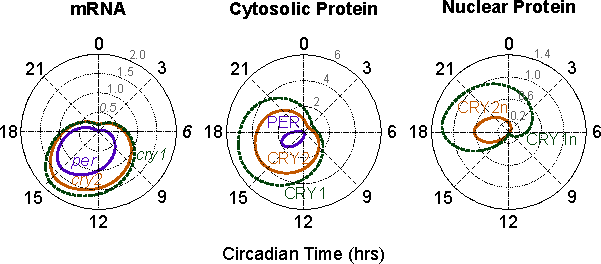
\includegraphics[width=0.8\textwidth]{chap2/figures/timecourse.pdf}
  \titlecaption{Time course concentration profiles of \fref{mod:hirota}}{
    The three polar plots show the time-varying levels of each clock component for optimal parameter set. 
    In these plots, the amplitude of each variable (always positive) is plotted against its phase, $0 \rightarrow 2\pi$. 
    Since the limit cycle is periodic, this results in a closed curve. 
    Rising mRNA levels caused by low repressor concentrations (CT12) result in accumulating cytosolic protein (left plot). 
    Lower levels of PER prevent all the available CRY from entering the nucleus (middle plot). 
  High levels of nuclear repressors halt transcription until both CRYs have degraded (right plot).}
  \label{fig:timecourse}
\end{figure}

\subsubsection{SiRNA knockdowns}
SiRNA knockdowns were performed {\it in silico} by increasing the degradation rate for the corresponding mRNA (\fref{fig:experimentalvalidation}), as done previously in \cite{Relogio2011}. 
{\it Cry1} and {\it Cry2} knockdowns in wild type conditions show close agreement to experiment \cite{Zhang2009}, and demonstrate that altering the nuclear CRY1/CRY2 ratio is effective in changing the period of oscillation.

\subsubsection{CRY2 cytosolic stabilization}
The {\it Dyrk1a} knockdown in \cite{Kurabayashi2010} serves as another demonstration of the change in period as a response to a change in nuclear CRY1/CRY2 ratio. 
To demonstrate the effect in silico, the degradation rate of cytosolic CRY2 was decreased. 
Matching experimental evidence, the cytosolic CRY2 levels rose, with a corresponding change in the nuclear CRY ratio and decrease in period.

\subsubsection{Single cry perturbations}
The $\text{\it Cry1}^{+/-}$ $\text{\it Cry2}^{-/-}$ and $\text{\it Cry1}^{-/-}$ $\text{\it Cry2}^{+/-}$ single/double knockout perturbations from \cite{VanderHorst1999} were approximated with an appropriate knockout and siRNA knockdown, and show the correct period shortening. 
With one {\it Cry} knocked out, the levels of cytoplasmic PER are no longer stoichiometrically limiting. 
In this case, less {\it Cry} leads to less nuclear complex, which is cleared faster.

\begin{figure}[bt]
  \centering
  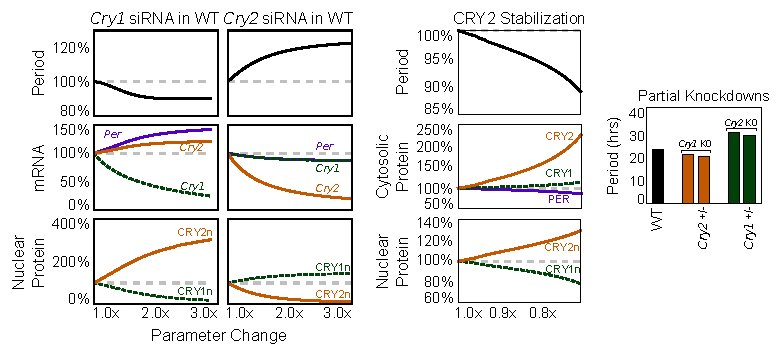
\includegraphics[width=\textwidth]{chap2/figures/experimentalvalidation.pdf}
  \titlecaption{Model validation against experimental results}{
    When comparing against existing experimental results, the model shows the correct response for {\it Cry1} siRNA, {\it Cry2} siRNA, and $\text{CRY}_c$ stabilization (left, middle), through an adjustment in the nuclear CRY1/CRY2 ratio. 
    The model also correctly captures the single/double knockout phenotype of \cite{VanderHorst1999}, (right)} \label{fig:experimentalvalidation}
\end{figure}

\subsection{Prediction of KL001 mechanism}
Using the completed model, we investigated possible mechanisms by which KL001 might lengthen the circadian period. 
Experimental evidence indicates that stabilization of CRY can either lengthen the period ({\it Fbxl3} knockdown) or shorten the period ({\it Dyrk1a} knockdown). 
Assuming equal effect on both isoforms of CRY, the model confirms that cytoplasmic stabilization results in period shortening, since excess CRY expedites the nuclear import of the PER:CRY repressive complex. 
However, stabilizing nuclear CRY (\fref{fig:nucleartimecourse}, last column) yields the appropriate period lengthening observed experimentally. 
We therefore predicted that KL001 acts primarily in the nucleus, potentially through the FBXL3 degradation pathway. 
Additionally, the model predicts that the compound’s effect on $\text{\it Cry1}^{-/-}$ and $\text{\it Cry2}^{-/-}$ systems would be similar to its effect on the wild type clock, causing dose-dependent period lengthening (\fref{fig:40662prediction}, left and right).


\begin{figure}[bt]
    \centering
    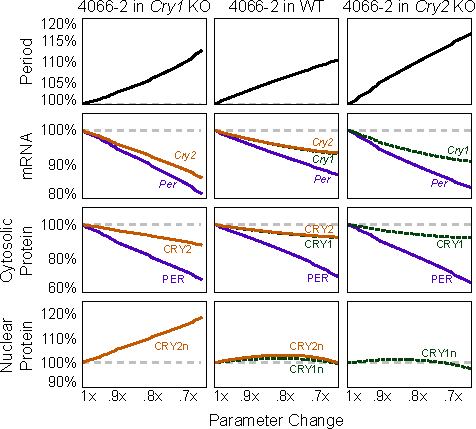
\includegraphics[width=0.7\textwidth]{chap2/figures/prediction.pdf}
    \titlecaption{Prediction of the KL001 mechanism}{ {\it In silico} response to equal stabilization of both CRYs in the nucleus results in longer periods (middle column), matching observed results. The model correctly predicts that stabilization of individual CRYs in the knockout environments also causes period lengthening.}
    \label{fig:40662prediction}
\end{figure}

\subsubsection{Experimental confirmation}
Experimental tests of the model's predictions were performed. 
Nuclear CRY1 and CRY2 levels were up-regulated and almost sustained, respectively, while PER1 level was strongly down-regulated by the compound, supporting stabilization of nuclear CRY, the predicted mechanism. 
Additionally, continuous treatment with KL001 lengthened the period in both {\it Cry1} and {\it Cry2} knockout cells in a dose-dependent manner. 
Similarly, the compound caused period lengthening in both CRY1 and CRY2 knockdown U2OS cells. 
We further investigated the effect of KL001 in SCN explants, which show robust rhythms even in the absence of {\it Cry1}, due to intercellular coupling \cite{Liu2007}. 
Both {\it Cry1} and {\it Cry2} knockout SCN exhibited dose-dependent period lengthening by the compound treatment. 
Thus, in a single {\it Cry} knockout, stabilization of either nuclear CRY1 and CRY2 causes period lengthening, confirming model predictions.
Furthermore, the period-lengthening response of KL001 was abolished in cells treated with FBXL3 siRNA, further confirming that the period effect of KL001 is mediated by inhibiting FBXL3-CRY interactions (\fref{fig:fbxl3data}).
This prediction was further verified in subsequent structural biology work \cite{Nangle2013}.

\begin{figure}[tbp]
  \centering
  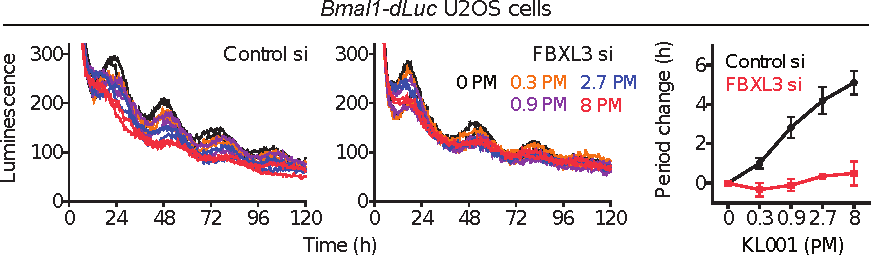
\includegraphics{chap2/figures/fbxl3kl001data.pdf}
  \titlecaption{FBXL3 knockdown interferes with period-lengthening effect of KL001}{The dose-dependent period increase of KL001 (right, black line) is abolished in cells treated with FBXL3 siRNA, indicating the mechanism of KL001 acts through FBXL3 and confirming model predictions}
  \label{fig:fbxl3data}
\end{figure}

\begin{figure}[p]
  \centering
  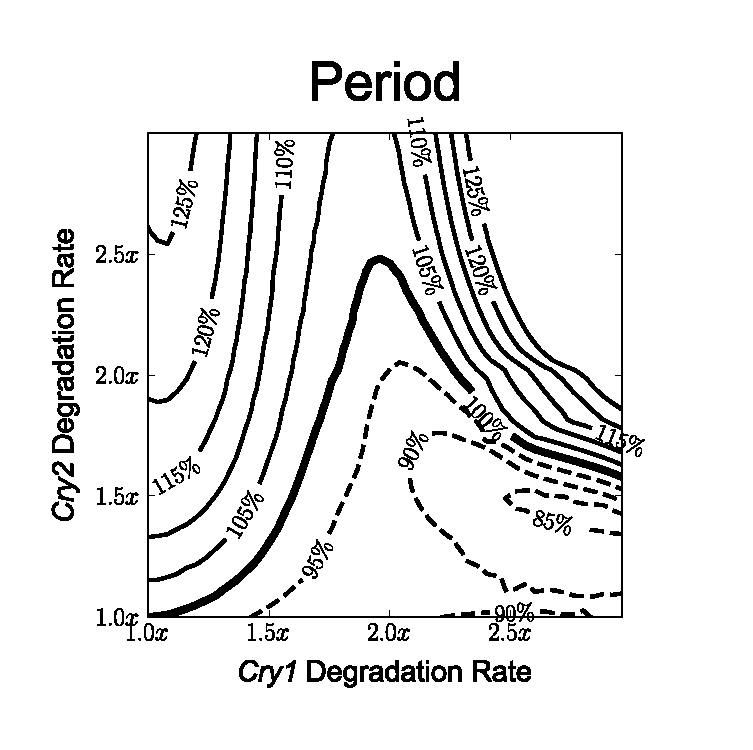
\includegraphics[width=0.5\textwidth]{chap2/figures/crysimultaneousknockdown.pdf}
  \titlecaption{Simultaneous knockdown of {\it Cry1} and {\it Cry2}}{Period contours (\% change) resulting from simultaneous {\it in silico} siRNA knockdowns of {\it Cry1} (x-axis) and {\it Cry2} (y-axis). The plot shows that the CRY1/CRY2 ratio determines the period, independent of total CRY, for perturbations up to twice the normal mRNA degradation rate.}
  \label{fig:simultaneouskdown}
\end{figure}

\begin{figure}[p]
  \centering
  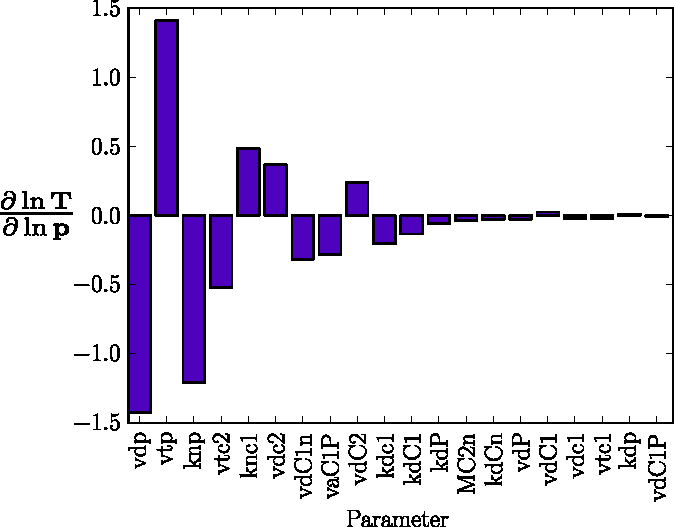
\includegraphics[width=0.6\textwidth]{chap2/figures/firstordersens.pdf}
  \titlecaption{First order relative period sensitivities}{ Dimensionless period sensitivities with respect to the kinetic parameters in the degradation-based model. Perturbations to most clock rates result in noticeable changes to the free-running period. Many of the most sensitive parameters are transcriptional rates, which can be easily changed through mutation of DNA promoter regions.}
  \label{fig:firstordersens}
\end{figure}

\section{Discussion}
\subsection{Insights into circadian network design}
Mathematical modeling has revealed how the balancing of two redundant feedback loops can provide fine control over the oscillatory period. 
A contour plot of period vs CRY1 or CRY2 abundance is shown in \fref{fig:simultaneouskdown}, which shows that the model's period is largely insensitive to the total amount of CRY ($45^\circ$ line), but highly dependent on the ratio of the two isoforms. 
Sensitivity analysis of our mathematical model (\fref{fig:firstordersens}) reveals that subtle changes in most of the involved rates can have an effect on the clock's free running period, which could be caused by evolutionary noise. 
Since many studies have linked entrainment to non-natural periods with long-term health problems, a mechanism to align the clock’s natural period to that of the environment would be advantageous. 
It is therefore possible that the period control afforded by CRY1/CRY2 balancing is a deliberately conserved design principle of the circadian clock, which confers period robustness against random mutations of clock components. 
Indeed, the presence of independent control of the cytosolic CRY2 levels suggests that the biological clock can control its period through simple post-translational modifications \cite{Kurabayashi2010}. 

\subsection{Identifiability of model parameters}
Due to the high dimensionality of the model equations and sparsity of the experimental data, it is likely that more than one set of parameters would fit the cost function defined in \fref{tab:cost}. 
While the fact that {\itshape any} parameter set for the given model equations reproduces experimental results is enough to confirm that our hypothesized mechanism is mathematically consistent, we must be careful in placing too much confidence in predictions based on the particular parameter set generated by the optimization algorithm. 
While subsequent experimental results confirm many of our model predictions, a more rigorous exploration of parameter space would allow us to determine which predictions are constrained by the available experimental data. 
However, incorporating error ranges via standard techniques such as bootstrap techniques are infeasible when using a genetic algorithm optimization strategy. 
In \fref{chap:id}, we describe techniques to improve computational efficiency to allow a more systematic evaluation of predictive confidence.
